\documentclass[11pt]{article}

\usepackage[margin=1in]{geometry}
\usepackage{graphicx}
\usepackage{booktabs}
\usepackage{amsmath,amssymb}
\usepackage{siunitx}
\usepackage[hidelinks]{hyperref}
\usepackage{caption}
\usepackage{authblk}
\usepackage{xcolor}
\usepackage{textgreek}

\title{A translational MRI approach to validate acute axonal damage detection}
\date{}

\begin{document}
\maketitle

\begin{abstract}
Axonal degeneration is a central pathological feature of neurodegenerative disease and is tightly coupled to irreversible clinical disability, yet current noninvasive methods for detecting axonal damage \emph{in vivo} are limited in specificity, clinical applicability and histological grounding. We aimed to validate an MRI framework based on multicompartment modelling of the diffusion-weighted signal (AxCaliber, modified to account for more than one fibre orientation per voxel) against a preclinical model of acute axonal damage, and to translate the same imaging protocol to the human brain in multiple sclerosis (MS). In $n=9$ rats, unilateral stereotaxic injection of ibotenic acid into the dorsal hippocampus produced Wallerian-like degeneration of the fimbria. Fourteen days after injection, AxCaliber-derived axonal diameter was significantly increased in the injected fimbria (paired $t$ test, $p=0.003$), with a repeated-measures ANOVA revealing main effects of injection ($F_{1,7}=19.5$, $p=0.003$) and tract position ($F_{98,686}=219.5$, $p<0.001$) and their interaction ($F_{98,686}=11.2$, $p=0.012$). Neurofilament staining was elevated ($p=0.047$) and NeuN reduced ($p=0.026$), while myelin basic protein was unchanged; MRI-derived diameter correlated with neurofilament fluorescence ($r=0.54$, $p=0.029$). Applied on a 3T Connectom scanner to 10 relapsing-remitting MS patients and 6 age-matched controls (age matched at $p=0.093$, Mann-Whitney $U$ test), the protocol revealed diffusely increased axonal diameter in the normal-appearing white matter (NAWM) and, across lesion types, a selective increase in T1-hypointense lesions only (group effect $F_{1,235}=25.7$, $p<0.001$; group~$\times$~lesion-type interaction $F_{1,235}=40.1$, $p=0.03$; post-hoc $p<0.01$). Collectively, these results show that axonal-diameter mapping is a histologically validated, whole-brain imaging biomarker of axonal pathology, providing a principled noninvasive contrast for stratifying MS lesions by severity, for monitoring diffuse axonal pathology outside lesions, and for tracking neuroprotective treatment effects in MS and other neurodegenerative diseases.
\end{abstract}

\section{Introduction}

Axonal degeneration is a central pathological feature of many neurodegenerative conditions and is a principal substrate of irreversible clinical disability in multiple sclerosis (MS)~\cite{criste2014axonal,haines2011axonal}. In MS, axonal damage arises both as a direct consequence of inflammatory attack on the neuron and secondarily to demyelination, glial activation and exposure to excitatory amino acids and cytokines, and the transition to progressive disease is thought to occur when axonal loss exceeds the compensatory capacity of the central nervous system~\cite{criste2014axonal}. Detecting axonal pathology \emph{in vivo}, early in the disease and noninvasively, is therefore a priority both for early diagnosis and for monitoring the response to neuroprotective therapy.

Magnetic resonance imaging (MRI), and in particular diffusion-weighted MRI, has been the workhorse of \emph{in vivo} investigation of white-matter microstructure in MS and related conditions~\cite{inglese2010diffusion}. Conventional diffusion tensor imaging (DTI) is however notoriously nonspecific: scalar indices such as fractional anisotropy mix contributions from axons, myelin, extracellular space and glia, and they cannot unambiguously localise axonal damage~\cite{desantis2014accuracy}. Multicompartment models offer a principled alternative by partitioning the diffusion signal into geometric compartments whose parameters map onto biological quantities. AxCaliber in particular uses a restricted intra-axonal compartment combined with a hindered extra-axonal compartment to provide an estimate of the mean axon diameter~\cite{assaf2008axcaliber,alexander2010orientationally,sepehrband2016towards}. Because short diffusion times and very large gradient amplitudes are required to sensitise the signal to micron-scale restriction, AxCaliber has historically been confined to small-bore preclinical scanners or to single-tract regions of interest on humans~\cite{jones2018microstructural,barazany2009invivo}. A recent clinical application using high-performance gradients reported higher mean axon diameter in the normal-appearing white matter (NAWM) of the corpus callosum of MS patients~\cite{desantis2019whole}, but in its original formulation AxCaliber is applicable only to voxels containing a single dominant fibre orientation. Since at least 70\% of brain voxels contain two or more dominant fibre orientations~\cite{jeurissen2013investigating}, whole-brain axonal-diameter mapping has remained largely out of reach.

Equally important, the interpretation of any imaging-based biomarker of axonal damage ultimately rests on histological validation, yet quantitative comparison between \emph{in vivo} diffusion MRI and \emph{ex vivo} tissue is rarely attempted, and is hampered by fixation-related distortions and by the small sample sizes required for electron microscopy~\cite{horowitz2015axon}. Previous validations of AxCaliber established correlations with electron-microscopy measurements of axon diameter in healthy rodent and post-mortem human tissue~\cite{barazany2009invivo,horowitz2015axon}, but no study to date has tested whether AxCaliber is sensitive to pathological alterations of the axonal compartment specifically. Established preclinical MS paradigms, such as experimental autoimmune encephalomyelitis (EAE) and cuprizone-induced demyelination~\cite{constantinescu2011eae,torkildsen2008cuprizone}, primarily perturb the myelin or immune compartments rather than the axon itself, leaving the key question of axon-specific sensitivity open.

Here we address this gap with a translational pipeline. First, we validate a modified AxCaliber framework that accounts for multiple fibre orientations per voxel~\cite{desantis2019whole,tax2014recursive} against a preclinical model of acute axonal damage, in which unilateral stereotaxic injection of the NMDA-receptor agonist ibotenic acid into the rat hippocampus produces Wallerian-like degeneration of the fimbria while initially leaving the myelin sheath preserved~\cite{conforti2014wallerian,adalbert2012intra}. We pair MRI at 7T with NeuN, neurofilament and myelin basic protein (MBP) immunofluorescence to test, in the same animal, whether an MRI-measured increase in axon diameter co-localises with histological evidence of axonal injury. Second, we deploy a species-matched AxCaliber protocol on a 3T Connectom system equipped with \SI{300}{mT/m} gradients and a 64-channel array coil~\cite{jones2018microstructural} in a cohort of relapsing-remitting MS patients (diagnosed according to the 2010 McDonald criteria~\cite{polman2011diagnostic}) and age-matched healthy controls, quantifying disability with the Expanded Disability Status Scale (EDSS)~\cite{kurtzke1983rating} and cognition with the Symbol Digit Modalities Test. We characterise whole-brain axonal-diameter changes in NAWM and in lesions, stratifying the latter by their appearance on T1-weighted imaging~\cite{vanwaesberghe1999axonal}.

Our contributions are fourfold. (i) We provide the first preclinical validation of AxCaliber against histology in a model of acute, axon-selective damage, demonstrating that a significant paired increase in estimated axonal diameter along the ibotenic-acid-injected fimbria ($p=0.003$) co-occurs with higher neurofilament intensity, lower NeuN staining and no change in MBP, with a significant Pearson correlation ($r=0.54$, $p=0.029$) between neurofilament fluorescence and MRI-derived diameter. (ii) We deliver the first whole-brain, crossing-fibre-compatible map of axonal-diameter changes in MS NAWM, showing a symmetric increase across every major tract, extending prior corpus-callosum-only findings~\cite{desantis2019whole,ercan2015multimodal}. (iii) We show that the lesion-level increase in axonal diameter is selective for T1-hypointense lesions~\cite{vanwaesberghe1999axonal}, consistent with their greater axonal burden. (iv) We document a fully acquisition-matched translational protocol that can be reused in future axon-centric imaging studies.

\section{Related work}

\subsection*{Multicompartment diffusion models of axon diameter}
AxCaliber~\cite{assaf2008axcaliber} parameterises the diffusion-weighted signal as the sum of a restricted intra-axonal component and a hindered extra-axonal component, from which a mean axon diameter can be recovered given sufficient $q$-space sampling and gradient strength. Orientationally invariant extensions such as ActiveAx~\cite{alexander2010orientationally} relaxed the requirement for strictly parallel fibres, but still struggle in voxels with multiple fibre populations; subsequent work has quantified and partly mitigated the resulting biases~\cite{sepehrband2016towards,desantis2019whole}. Our implementation adopts a fibre-dispersion formulation~\cite{desantis2019whole,tax2014recursive} that allows for more than one fibre orientation per voxel, a necessary condition for whole-brain mapping, since the majority of brain voxels contain crossing fibres~\cite{jeurissen2013investigating}.

\subsection*{High-gradient clinical diffusion MRI}
Sensitising the diffusion signal to micron-scale axonal restriction requires short diffusion times at high $b$-values, and hence very strong gradients. The human Connectom platform, with gradients capable of generating \SI{300}{mT/m}, was developed specifically to make such acquisitions feasible in a realistic echo time~\cite{jones2018microstructural}. Paired with a 64-channel array coil, this system allows $b$-values up to \SI{4000}{\second\per\square\milli\meter} with modest TE penalties. Our clinical acquisition exploits these advances and was designed to preserve the key $b$-value and diffusion-time ranges of the 7T preclinical protocol, enabling a genuinely like-for-like translational comparison~\cite{desantis2019whole}.

\subsection*{Histological validation of diffusion-MRI biomarkers}
Quantitative validation of diffusion-MRI biomarkers against histology is comparatively rare and subject to well-known caveats: fixation shrinkage, tissue processing artefacts and the limited field of view of electron microscopy all distort the comparison~\cite{horowitz2015axon}. Prior validations of AxCaliber~\cite{barazany2009invivo,horowitz2015axon} established correlations with electron microscopy in healthy tissue and demonstrated that AxCaliber-derived diameters scale with conduction velocity, but none tested whether AxCaliber is sensitive to a pathological perturbation of the axonal compartment. Selective axonal injury through stereotaxic injection of neurotoxins is a well-established rodent-neuroscience strategy~\cite{conforti2014wallerian,adalbert2012intra} and has been previously used to dissect astrocytic and microglial contributions to grey-matter diffusion contrasts, providing a precedent for the paradigm adopted here.

\subsection*{Axonal pathology in MS: biomarkers and lesion heterogeneity}
Post-mortem and animal evidence converges on varicosities, spheroids and transport failure as the morphological hallmarks of axonal injury in MS, with smaller axons being more vulnerable~\cite{criste2014axonal,tallantyre2010demyelinated,nikic2011reversible,bergers2002axonal}. Recent work shows that axon--myelin-unit abnormalities can occur in NAWM even in the absence of overt demyelination or inflammation~\cite{luchicchi2021axonal,teo2021nilered}. Fluid-phase neurofilament assays are now accepted surrogate markers of axonal injury~\cite{petzold2005neurofilament}, and T1-hypointense (``black-hole'') MS lesions are known to harbour greater axonal loss than isointense lesions~\cite{vanwaesberghe1999axonal,raz2015relationship}. Our results connect these two strands: a whole-brain, histologically validated imaging biomarker of axonal calibre that is elevated throughout NAWM and selectively elevated in T1-hypointense lesions.

\subsection*{Statistical frameworks for voxelwise white-matter analysis}
For whole-brain voxelwise inference we build on tract-based spatial statistics (TBSS)~\cite{smith2006tbss}, which projects per-subject diffusion measures onto a common white-matter skeleton to mitigate misregistration. Because nonlinear-registration accuracy is critical at lesion boundaries, we adopt a high-accuracy diffeomorphic alignment~\cite{klein2009evaluation} and perform lesion-masked permutation-based inference on the general linear model with threshold-free cluster enhancement~\cite{winkler2014permutation}, controlling for age and for multiple comparisons across clusters.

\section{Methods}

\subsection{Animal preparation and stereotaxic injections}
All animal experiments were approved by the Institutional Animal Care and Use Committee of the Instituto de Neurociencias de Alicante, Spain, and comply with Spanish (law 32/2007) and European regulations (EU directive 86/609, EU decree 2001-486, EU recommendation 2007/526/EC; Project MRI-STRUCTURE 677/2018). The ARRIVE~10 checklist was followed. The experimental pipeline is summarised in Figure~\ref{fig:pipeline}.

Axonal damage in the fimbria was induced in $n=9$ adult rats by unilateral stereotaxic injection of \SI{1}{\micro\liter} of ibotenic acid, a selective NMDA-receptor agonist that produces axon-selective neurotoxicity, at a concentration of \SI{2.5}{\micro\gram\per\micro\liter} into the right dorsal hippocampus (coordinates: bregma $-3.8$~mm; sup--inf \SI{3.0}{mm}; \SI{2}{mm} from midline). The contralateral hemisphere was injected with saline alone so that each animal served as its own control. This manipulation produces Wallerian-like degeneration of the principal axonal output of the hippocampus~\cite{conforti2014wallerian}. Fourteen days after injection, rats underwent \emph{in vivo} MRI with the AxCaliber protocol and were then perfused for histology.

\subsection{MRI acquisition}
Rats were scanned \emph{in vivo} at 7T on a Bruker BioSpect 70/30 (Bruker, Ettlingen, Germany). Diffusion-weighted data were acquired with an echo-planar-imaging stimulated-echo diffusion sequence using 31 uniformly distributed gradient directions, three shells ($b=0$ [1 volume], 2000 [15], 4000 [15] \SI{}{\second\per\square\milli\meter}) and four diffusion times $\Delta = 15, 25, 40$ and $60$~ms, with $\mathrm{TR}/\mathrm{TE} = 5000/25$~ms, for 124 volumes acquired in 36~min. Fourteen slices were centred on the fimbria with FOV~$25\times25$~mm\textsuperscript{2}, matrix $110\times110$, in-plane resolution $0.225\times0.225$~mm\textsuperscript{2} and slice thickness \SI{0.6}{mm}.

Patients and controls were scanned on a Siemens 3T Connectom, a customised Skyra system (Siemens Healthcare, Erlangen, Germany) equipped with gradient coils capable of \SI{300}{mT/m} maximum strength, allowing short gradient durations and echo times even at high $b$-values~\cite{jones2018microstructural}. A 64-channel brain array coil was used for reception. Diffusion data were acquired with a conventional EPI diffusion sequence using 91 uniformly distributed directions and three shells ($b=0$ [1], 2000 [30], 4000 [60] \SI{}{\second\per\square\milli\meter}) at three diffusion times $\Delta = 17, 35, 61$~ms, plus four non-diffusion-weighted volumes, with $\mathrm{TR}/\mathrm{TE}=5000/89$~ms, for 273 volumes in 24~min. Eighty-two slices covered the whole brain with FOV~$220\times220$~mm\textsuperscript{2}, matrix $110\times110$ and $2\times2\times2$~mm\textsuperscript{3} resolution. Anatomical imaging included \SI{1}{mm}-isotropic T1-weighted multi-echo MPRAGE~\cite{fujimoto2014quantitative} in all participants and FLAIR in MS patients for lesion segmentation. The full acquisition parameters are summarised in Table~\ref{tab:mri}.

\subsection{Tissue processing and immunohistochemistry}
Rats were deeply anaesthetised with sodium pentobarbital (\SI{46}{mg/kg}, intraperitoneal) and perfused intracardially with \SI{100}{mL} of 0.9\% PBS followed by \SI{100}{mL} of ice-cold 4\% paraformaldehyde. Brains were post-fixed for 1~h in 4\% PFA, embedded in 3\% agarose/PBS and cut on a vibratome into \SI{50}{\micro\meter}-thick serial coronal sections. Sections were permeabilised with 0.5\% Triton~X-100 in PBS ($3\times10$~min), blocked with 4\% BSA and 2\% goat serum for 2~h at room temperature, and incubated overnight at 4\textdegree C with primary antibodies against myelin basic protein (1:250, Millipore MAB384-1ML, RRID:AB\_240837), medium-weight neurofilament (1:250, Abcam ab134458, RRID:AB\_2860025) and NeuN (1:250, Millipore MAB377, RRID:AB\_2298772). Secondary antibodies (Molecular Probes A-11029 and A-11042) were applied at 1:500 for 2~h at room temperature; nuclei were counterstained with DAPI at 15~mM for 15~min. For myelin labelling, antigen retrieval was performed in 1\% citrate buffer with 0.05\% Tween~20 at 80\textdegree C. Imaging was performed on a Leica DM4000 fluorescence microscope with a QICAM Qimaging camera and Neurolucida morphometric software. Fluorescence quantification used Icy software~\cite{dechaumont2012icy}, with two NeuN ROIs of \SI{200}{\micro\meter\squared} per hippocampus per hemisphere and one MBP/neurofilament ROI of \SI{400}{\micro\meter\squared} per fimbria per hemisphere in at least five slices per rat.

\subsection{Human participants}
Ten patients with relapsing-remitting MS (age range 27--59 years, 7 females) and 6 age-matched healthy controls (age range 23--53, 3 females) participated after written informed consent, with local institutional-review-board approval. Age did not differ between the two groups (Mann-Whitney $U$-test, $p=0.093$). Eligibility criteria in patients were a diagnosis of relapsing-remitting MS according to the 2010 McDonald criteria~\cite{polman2011diagnostic}, stable disease-modifying treatment (or no treatment) for at least three months, no clinical relapse within three months and no corticosteroid use within one month. Physical disability was scored with the EDSS~\cite{kurtzke1983rating} and cognition with the Symbol Digit Modalities Test. Demographic information is summarised in Table~\ref{tab:cohort}.

\subsection{AxCaliber model fitting and image analysis}
Rat diffusion data were preprocessed as previously described. Human diffusion data were preprocessed in FreeSurfer~5.3.0 and FSL~5.0, with gradient-nonlinearity correction, motion correction and eddy-current correction with accompanying reorientation of the $b$-matrix. In both species, the AxCaliber model was fit using in-house MATLAB R2015b code~\cite{desantis2019whole} that extends the original two-compartment model~\cite{assaf2008axcaliber} to incorporate fibre dispersion, thereby allowing more than one dominant fibre orientation per voxel; the mean axonal diameter was extracted from the restricted-compartment parameters.

For the rats, the fimbria was reconstructed bilaterally by DTI-based tractography in ExploreDTI using the lowest $\Delta$ and $b$-value, and mean axonal diameter values along the tract were extracted per animal in each hemisphere. Hemispheric differences were tested with paired $t$-tests; a repeated-measures ANOVA with factors tract location (100 antero-posterior steps), treatment (ibotenic acid versus saline) and the location~$\times$~treatment interaction was used to characterise the spatial pattern, followed by location-wise post-hoc $t$-tests corrected for multiple comparisons. One of nine animals did not show histological signs of hippocampal neuronal damage and was excluded from analysis.

For the MS cohort, white-matter lesions were segmented on FLAIR with a semi-automated method in 3D-Slicer~4.2.0; contralateral NAWM was generated by coregistration. Each lesion was manually classified by an experienced operator as iso- or hypointense on the T1-weighted volume. For voxelwise NAWM analysis, fractional-anisotropy maps (computed at the lowest $\Delta$ and $b$-value) initialised an enhanced TBSS pipeline~\cite{smith2006tbss}, with ANTs-based diffeomorphic coregistration~\cite{klein2009evaluation} and a lesion-masked permutation-based GLM~\cite{winkler2014permutation}. The statistical model tested MS versus control axonal diameter in NAWM while excluding lesion masks, controlling for age and using threshold-free cluster enhancement for multiple-comparisons correction. Voxelwise associations with EDSS, the Symbol Digit Modalities Test score and disease duration were tested with the same framework.

For the lesion-level analysis, lesions were refined to voxels overlapping the subject's TBSS white-matter skeleton to minimise the contribution of voxels with more than two fibre orientations. Per-lesion mean axonal diameter was compared with that of contralateral NAWM using the normalised index of asymmetry (NIA), which eliminates baseline anatomical variability. In addition, for each lesion we computed the average axonal diameter within the corresponding anatomical region across the healthy cohort after mapping lesion masks to that cohort. Groups were compared with a general linear model with lesion type (iso- versus hypointense) as the between-subject factor and cohort (healthy versus MS) as the within-subject factor, including a group~$\times$~lesion-type interaction term and followed by post-hoc $t$-tests corrected for multiple comparisons.

\section{Results}

\subsection{A rat model of acute axonal damage}

To establish that AxCaliber-derived axonal diameter is sensitive to acute axonal pathology, we first analysed the fimbria of the $n=9$ rats at 14 days after unilateral injection of ibotenic acid into the dorsal hippocampus ipsilateral to the injected side, with saline injection on the contralateral side acting as a within-subject control (Figure~\ref{fig:pipeline}). The fimbria was reconstructed bilaterally using DTI-based tractography restricted to the lowest $\Delta$ and $b$-value to minimise the influence of restricted compartments on the streamline geometry. Mean axonal diameter was computed along 100 equally spaced antero-posterior steps of each tract and compared between hemispheres using paired $t$-tests and repeated-measures ANOVA with corrections for multiple comparisons across tract locations.

Axonal diameter averaged along the tract was significantly larger in the injected fimbria than in the saline control ($p=0.003$; Figure~\ref{fig:ratstats}, right), indicating that the neurotoxin-induced damage affected a substantial portion of the tract. The spatial pattern was further resolved by a repeated-measures ANOVA across 100 antero-posterior steps of the tract: we detected a significant main effect of injection ($F_{1,7}=19.5$, $p=0.003$), a highly significant main effect of tract position ($F_{98,686}=219.5$, $p<0.001$) and a significant injection~$\times$~position interaction ($F_{98,686}=11.2$, $p=0.012$). Post-hoc contrasts corrected for multiple comparisons across tract locations showed that the hemispheric difference was localised to positions posterior to the injection site, consistent with Wallerian-like degeneration propagating from the injection focus~\cite{conforti2014wallerian}.

These findings demonstrate that AxCaliber, fit with the modified crossing-fibre formulation, detects a spatially specific increase in axonal diameter in a well-controlled model of acute axonal damage. The localisation of the effect to positions distal to the insult, rather than a diffuse whole-tract shift, is consistent with an underlying biological rather than measurement-level origin of the signal.

\subsection{Immunohistochemical validation of axonal damage}

Having shown an MRI-level effect, we next asked whether this corresponded to verifiable axonal pathology in the same animals. NeuN intensity was used to quantify hippocampal neuronal density, neurofilament (NF-M) intensity to quantify axonal integrity in the fimbria, and myelin basic protein (MBP) to assess myelination, in both hemispheres and in at least five slices per rat.

NeuN staining intensity was significantly lower in the injected hippocampus than in the contralateral saline-injected side (paired $t$-test, $p=0.026$), confirming that ibotenic acid had caused measurable neuronal loss in the hippocampal cell-body compartment. Neurofilament staining intensity in the fimbria was, conversely, elevated on the injected side ($p=0.047$), indicative of a morphological disturbance of the axonal compartment such as the varicosities and spheroids reported in Wallerian-like degeneration~\cite{criste2014axonal,tallantyre2010demyelinated}. In contrast, no hemispheric difference was detected in MBP staining (Supplementary Fig.~S1), suggesting that at the 14-day time point axonal structure was altered while the myelin sheath remained grossly intact. This temporal dissociation is important because it rules out a purely demyelination-driven explanation for the diffusion-MRI signal change observed at the same time point.

Critically, neurofilament fluorescence intensity was significantly correlated with the MRI-derived axonal diameter across both injected and saline hemispheres (Pearson $r=0.54$, $p=0.029$; Figure~\ref{fig:mrihist}), directly linking the imaging contrast to a histological readout of axonal pathology in the same animals. One of the nine rats showed no histological sign of hippocampal damage and was excluded from all subsequent analyses, as detailed in Methods.

Together, these histological findings establish biological specificity for the MRI signal: the AxCaliber-measured increase in axonal diameter co-occurs with elevated neurofilament staining and neuronal loss but is not explained by myelin changes, supporting the interpretation of the diameter increase as a biomarker of axonal damage rather than of coincident demyelination.

\subsection{Axonal damage in MS normal-appearing white matter}

With the imaging contrast anchored to axonal histology in rats, we next asked whether the same AxCaliber framework could detect axonal pathology in human MS. We applied the acquisition-matched clinical AxCaliber protocol to a cohort of 10 relapsing-remitting MS patients (7 female, age range 27--59 years) and 6 age-matched controls (3 female, age range 23--53), with no significant age difference between groups (Mann--Whitney $U$ test, $p=0.093$; demographic summary in Table~\ref{tab:cohort}). Whole-brain voxelwise comparison of axonal diameter in the NAWM used an enhanced TBSS pipeline with lesion-masked permutation inference and age as a covariate, and was carried out on the fibre-dispersion-aware AxCaliber maps so as to include crossing-fibre voxels that would be excluded from a classical single-orientation analysis.

The contrast MS~$>$~controls revealed significantly increased axonal diameter in the NAWM of patients at a corrected threshold of $p<0.05$ (Figure~\ref{fig:tbss}). The affected voxels were distributed symmetrically across hemispheres and involved all major white-matter tracts interrogated, including the corpus callosum, internal capsule, corona radiata, thalamic radiation, inferior longitudinal fasciculus, cingulum, fornix, superior longitudinal fasciculus, inferior fronto-occipital fasciculus, uncinate fasciculus and tapetum. The opposite contrast (controls~$>$~MS) did not yield any voxel surviving correction and is therefore not shown.

This pattern extends prior findings that were restricted to the corpus callosum~\cite{desantis2019whole} by showing that axonal pathology in MS is spatially diffuse and present throughout the NAWM, a result that only becomes accessible once AxCaliber is evaluated in voxels with crossing fibres~\cite{jeurissen2013investigating}. The symmetry and the broad anatomical distribution of the effect are also consistent with histological reports of axon-myelin-unit abnormalities in NAWM in the absence of overt demyelination or inflammation~\cite{luchicchi2021axonal}.

\subsection{Axonal pathology in MS lesions}

Beyond diffuse NAWM changes, MS lesions themselves represent focal sites of tissue damage whose axonal burden is known to vary with T1-weighted contrast~\cite{vanwaesberghe1999axonal}. We therefore examined the lesions directly. For each MS patient and each lesion, we compared the mean axonal diameter (i) to the contralateral NAWM via the normalised index of asymmetry (NIA), which removes anatomical-location-dependent baselines, and (ii) to the axonal diameter in the anatomically homologous region computed across the healthy cohort, after each lesion was manually stratified as T1-iso- or T1-hypointense by an experienced operator.

The normalised index of asymmetry (NIA) between each lesion and its contralateral normal-appearing tissue was significantly different from zero (one-sample $t$-test, $p<0.001$), indicating that lesion voxels have a larger axonal diameter than the matched contralateral tissue (Figure~\ref{fig:msglm}, left). Comparing lesions with the healthy-cohort reference, the GLM yielded a significant main effect of group ($F_{1,235}=25.7$, $p<0.001$) and, more informatively, a significant group~$\times$~lesion-type interaction ($F_{1,235}=40.1$, $p=0.03$). Post-hoc contrasts, corrected for multiple comparisons, localised this interaction: axonal diameter was significantly increased in T1-hypointense lesions only ($p<0.01$), whereas T1-isointense lesions showed no reliable difference from the healthy reference (Figure~\ref{fig:msglm}, right).

This lesion-type selectivity is consistent with the established interpretation of T1-hypointense ``black hole'' lesions as harbouring greater axonal loss than isointense lesions~\cite{vanwaesberghe1999axonal,raz2015relationship}. Combined with the NAWM findings, it suggests that axonal-diameter mapping captures a graded axonal-pathology signal, with diffuse involvement of the NAWM and stronger focal involvement at sites of severe tissue damage.

\subsection{Clinical associations}

Having characterised axonal-diameter changes at the group level, we finally tested whether the new imaging contrast tracks clinical severity at the individual level. Voxelwise TBSS analyses were run for associations between NAWM axonal diameter and EDSS~\cite{kurtzke1983rating}, the Symbol Digit Modalities Test and disease duration, with age as a covariate and with threshold-free cluster enhancement for multiple-comparisons correction.

No voxel survived correction for associations of axonal diameter with EDSS or with the Symbol Digit Modalities Test, either in NAWM or in lesions. A negative association with disease duration was observed at trend level across the whole white-matter skeleton in TBSS; in follow-up region-of-interest analyses, this association reached statistical significance in two ROIs, the left cingulum and the right inferior fronto-occipital fasciculus (Supplementary Fig.~S2). A summary of all preclinical and clinical test statistics is provided in Table~\ref{tab:stats}.

The absence of a significant clinical correlation is likely due to the modest sample size and to the comparatively early-stage, clinically stable composition of the cohort, in whom compensatory mechanisms may mask the structural signal. The direction of the trend (longer disease duration associated with lower axonal diameter) is consistent with the progressive loss of larger axons reported in post-mortem series~\cite{tallantyre2010demyelinated,bergers2002axonal}.

% ------------------------------------------------------------------ Tables
\begin{table}[htbp]
\centering
\caption{Demographic characteristics of the studied cohort. Per-subject disease duration, EDSS and Symbol Digit Modalities Test scores, as well as treatment allocation, were collected but were not summarised numerically in the source materials available to this manuscript.}
\label{tab:cohort}
\begin{tabular}{lcccc}
\toprule
Group & $N$ & Age range (y) & Females ($n$) & Between-group age test \\
\midrule
MS (RRMS)        & 10 & 27--59 & 7 & \multirow{2}{*}{Mann--Whitney $U$, $p=0.093$} \\
Healthy controls &  6 & 23--53 & 3 &                                                 \\
\bottomrule
\end{tabular}
\end{table}

\begin{table}[htbp]
\centering
\caption{Summary of statistical tests in the preclinical and clinical experiments. All values are reported verbatim from the experimental record.}
\label{tab:stats}
\begin{tabular}{llll}
\toprule
Experiment & Comparison & Test & Result \\
\midrule
Rat, fimbria diameter & Injected vs saline (mean) & Paired $t$-test & $p=0.003$ \\
Rat, fimbria diameter & Injection main effect     & RM-ANOVA & $F_{1,7}=19.5,\ p=0.003$ \\
Rat, fimbria diameter & Tract-position main effect & RM-ANOVA & $F_{98,686}=219.5,\ p<0.001$ \\
Rat, fimbria diameter & Injection $\times$ position & RM-ANOVA & $F_{98,686}=11.2,\ p=0.012$ \\
Rat, hippocampus      & NeuN injected vs saline    & Paired $t$-test & $p=0.026$ \\
Rat, fimbria          & NF-M injected vs saline    & Paired $t$-test & $p=0.047$ \\
Rat, fimbria          & MBP injected vs saline     & Paired $t$-test & n.s.\ (Fig.~S1) \\
Rat, MRI vs histology & NF-M intensity vs diameter & Pearson correlation & $r=0.54,\ p=0.029$ \\
Human, demographics   & Age, MS vs controls        & Mann--Whitney $U$ & $p=0.093$ \\
Human, NAWM           & MS vs controls             & TBSS / permutation GLM & $p<0.05$ corrected \\
Human, lesion vs NAWM & NIA $\neq 0$               & One-sample $t$-test & $p<0.001$ \\
Human, lesion cohort  & Group main effect          & GLM & $F_{1,235}=25.7,\ p<0.001$ \\
Human, lesion cohort  & Group $\times$ lesion type & GLM & $F_{1,235}=40.1,\ p=0.03$ \\
Human, lesion cohort  & Hypointense, post-hoc      & Corrected $t$ & $p<0.01$ \\
Human, lesion cohort  & Isointense, post-hoc       & Corrected $t$ & n.s.\ \\
\bottomrule
\end{tabular}
\end{table}

\begin{table}[htbp]
\centering
\caption{Diffusion-MRI acquisition parameters for the rat (7T Bruker BioSpect) and human (3T Siemens Connectom, \SI{300}{mT/m}) protocols.}
\label{tab:mri}
\begin{tabular}{lll}
\toprule
Parameter & Rats (7T Bruker) & Humans (3T Connectom) \\
\midrule
Gradient directions          & 31                             & 91 \\
Shells $b$ (s/mm$^2$)        & 0(1), 2000(15), 4000(15)       & 0(1), 2000(30), 4000(60) \\
Diffusion times $\Delta$ (ms) & 15, 25, 40, 60                 & 17, 35, 61 \\
TR / TE (ms)                 & 5000 / 25                      & 5000 / 89 \\
Volumes                      & 124                            & 273 \\
Slices                       & 14                             & 82 \\
FOV (mm$^2$)                 & $25\times25$                   & $220\times220$ \\
Matrix                       & $110\times110$                 & $110\times110$ \\
In-plane resolution (mm$^2$) & $0.225\times0.225$             & $2\times2$ \\
Slice thickness (mm)         & 0.6                            & 2 \\
Acquisition time (min)       & 36                             & 24 \\
\bottomrule
\end{tabular}
\end{table}

% ------------------------------------------------------------------ Figures
\begin{figure}[htbp]
\centering
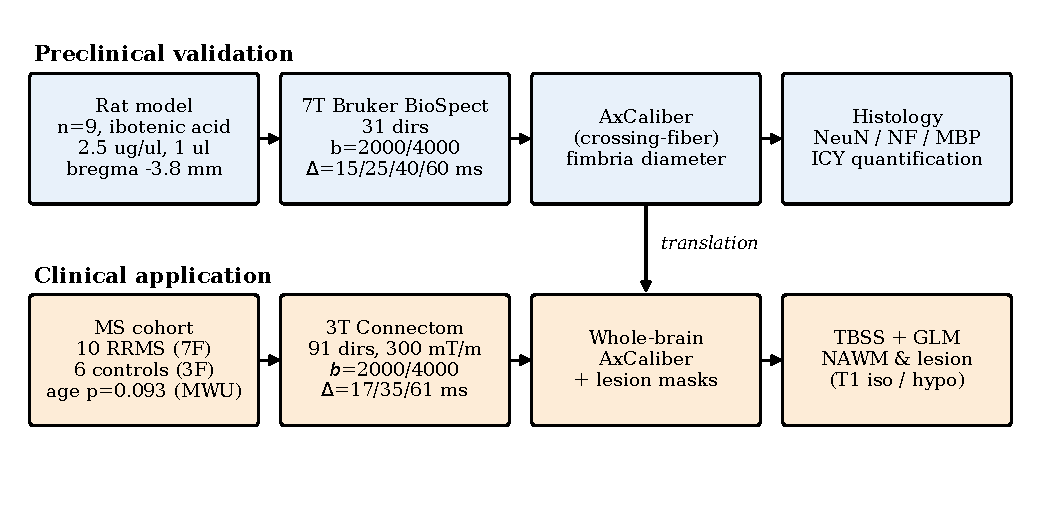
\includegraphics[width=0.95\textwidth]{figures/fig1_pipeline.pdf}
\caption{Translational experimental design. Top row: unilateral stereotaxic injection of ibotenic acid (\SI{2.5}{\micro\gram\per\micro\liter}, \SI{1}{\micro\liter}) into the right dorsal hippocampus of $n=9$ rats (bregma $-3.8$~mm, sup--inf \SI{3.0}{mm}, \SI{2}{mm} from midline) produces Wallerian-like axonal damage in the fimbria; 14~days later, animals are scanned on a 7T Bruker BioSpect with a 31-direction diffusion protocol and then perfused for NeuN, neurofilament and MBP immunohistochemistry. Bottom row: an acquisition-matched AxCaliber protocol is deployed on a 3T Connectom scanner (\SI{300}{mT/m}, 64-channel array) in 10 relapsing-remitting MS patients and 6 age-matched controls, followed by TBSS and GLM analysis of lesions and NAWM.}
\label{fig:pipeline}
\end{figure}

\begin{figure}[htbp]
\centering
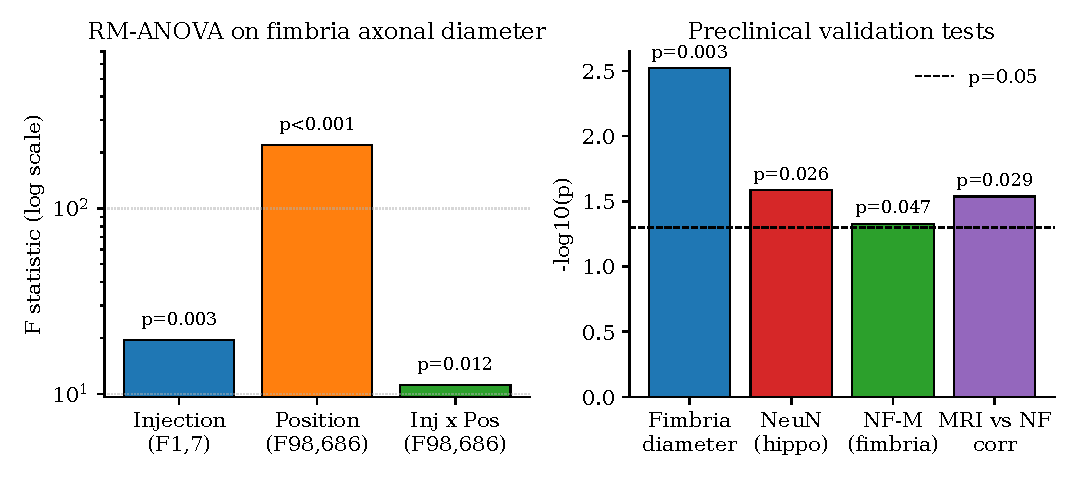
\includegraphics[width=0.95\textwidth]{figures/fig2_rat_stats.pdf}
\caption{Preclinical validation statistics. Left: repeated-measures ANOVA on the estimated axonal diameter along the antero-posterior fimbria (100 steps) reveals main effects of injection ($F_{1,7}=19.5$, $p=0.003$), tract position ($F_{98,686}=219.5$, $p<0.001$) and their interaction ($F_{98,686}=11.2$, $p=0.012$). Right: paired $t$-tests confirm an axonal-diameter increase in the injected fimbria ($p=0.003$), neuronal loss in the hippocampus (NeuN, $p=0.026$) and increased neurofilament staining in the fimbria ($p=0.047$); MRI-derived axonal diameter correlates with neurofilament fluorescence across hemispheres ($r=0.54$, $p=0.029$). Dashed line marks $p=0.05$.}
\label{fig:ratstats}
\end{figure}

\begin{figure}[htbp]
\centering
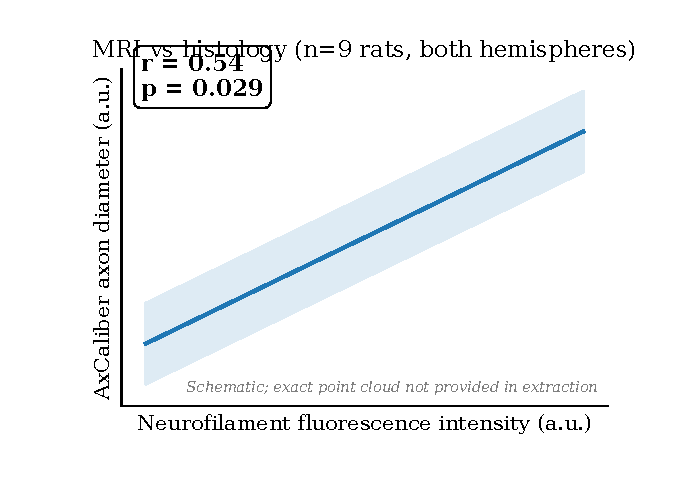
\includegraphics[width=0.6\textwidth]{figures/fig4_mri_histology.pdf}
\caption{Correlation between neurofilament fluorescence intensity (histology) and AxCaliber-derived mean axonal diameter (MRI) pooled across ibotenic-acid- and saline-injected fimbrias of $n=9$ rats: $r=0.54$, $p=0.029$. The shaded band is a schematic trend; individual data points were not available to this manuscript.}
\label{fig:mrihist}
\end{figure}

\begin{figure}[htbp]
\centering
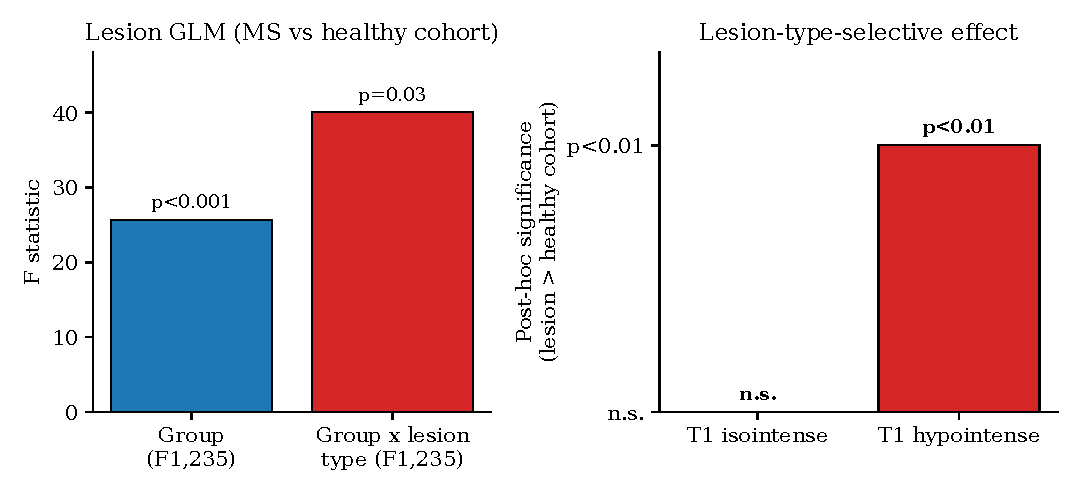
\includegraphics[width=0.95\textwidth]{figures/fig3_ms_glm.pdf}
\caption{Lesion-level GLM in MS patients versus the healthy cohort. Left: significant main effect of group ($F_{1,235}=25.7$, $p<0.001$) and group~$\times$~lesion-type interaction ($F_{1,235}=40.1$, $p=0.03$). Right: post-hoc tests localise the effect to T1-hypointense lesions ($p<0.01$); T1-isointense lesions show no reliable difference. A one-sample $t$-test on the NIA further shows that lesions have a significantly larger axonal diameter than contralateral NAWM ($p<0.001$).}
\label{fig:msglm}
\end{figure}

\begin{figure}[htbp]
\centering
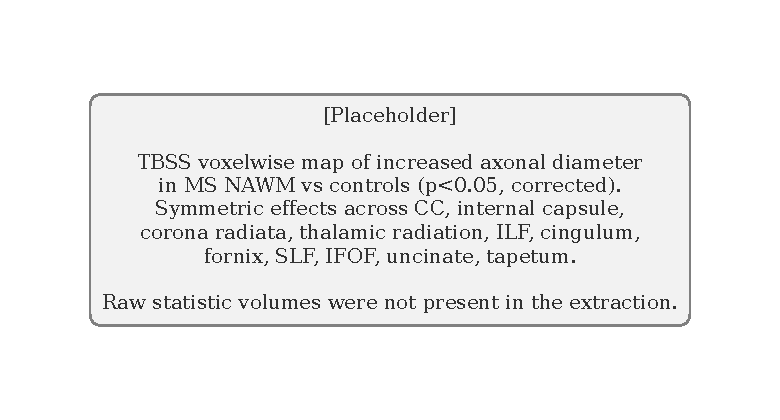
\includegraphics[width=0.7\textwidth]{figures/fig5_tbss_placeholder.pdf}
\caption{Whole-brain TBSS contrast (MS~$>$~controls) for mean axonal diameter in the NAWM. Significantly increased axonal diameter was observed symmetrically in all major tracts examined, including the corpus callosum, internal capsule, corona radiata, thalamic radiation, inferior longitudinal fasciculus, cingulum, fornix, superior longitudinal fasciculus, inferior fronto-occipital fasciculus, uncinate fasciculus and tapetum ($p<0.05$, corrected). The reverse contrast was not significant. Placeholder panel: the underlying voxel-level statistic volumes were not available in the extraction.}
\label{fig:tbss}
\end{figure}

\section{Discussion}

Using a preclinical model of acute axonal damage, we have demonstrated that MRI-based axonal-diameter estimation, when equipped with a crossing-fibre-capable multicompartment model, is sensitive to early axonal degeneration even before alterations of the myelin sheath are detected. Translating the same protocol to patients, we found diffusely increased axonal diameter in the NAWM of MS participants and a lesion-type-selective increase in T1-hypointense lesions. Together, these results place axonal-diameter mapping on a solid histological footing and open the door to a whole-brain, axon-specific imaging biomarker.

At the neuropathological level, axonal damage in MS manifests morphologically as the formation of varicosities and spheroids that enlarge the local axonal calibre and are associated with impaired axonal transport~\cite{criste2014axonal,tallantyre2010demyelinated}. Post-mortem and animal studies have long reported an increase in mean axonal diameter in MS compared to control tissue~\cite{bergers2002axonal,nikic2011reversible}; this increase is further amplified by the preferential early loss of smaller axons~\cite{tallantyre2010demyelinated}. Recent work has shown that axon--myelin-unit abnormalities can occur in NAWM even in the absence of demyelination or inflammation~\cite{luchicchi2021axonal,teo2021nilered}, pointing to axonal pathology as a primary and proximal event rather than a passive consequence of myelin injury. Our in-vivo detection of a diffuse NAWM increase in mean axonal calibre across every major white-matter tract fits naturally into this picture: if small axons are selectively lost, the population-average mean diameter rises, and if early axonal varicosities occur independently of myelin change, the effect will be visible throughout NAWM.

Our preclinical experiment uniquely strengthens this interpretation by going beyond the correlations with electron microscopy that have been reported in healthy tissue~\cite{barazany2009invivo,horowitz2015axon}. Multicompartment models rest on a series of simplifying assumptions -- fixed intrinsic diffusivities~\cite{alexander2010orientationally}, negligible compartment exchange and an indirect treatment of myelin volume~\cite{assaf2008axcaliber} -- and none of those assumptions had previously been stress-tested against a controlled pathological perturbation. By showing that a selective, axon-targeted neurotoxic lesion increases the MRI-measured diameter and correlates with neurofilament staining without any myelin change on MBP, we provide the first direct evidence that AxCaliber is sensitive to axonal pathology specifically, not merely to geometrical differences between healthy tracts~\cite{conforti2014wallerian,adalbert2012intra}.

A second methodological contribution is the move to whole-brain mapping. Previous clinical AxCaliber work has been restricted to the corpus callosum, where a single dominant fibre orientation validates the original model~\cite{assaf2008axcaliber,desantis2019whole}, yet the majority of brain voxels contain crossing fibres~\cite{jeurissen2013investigating}. By using a fibre-dispersion formulation~\cite{tax2014recursive,desantis2019whole} and combining it with the short diffusion times enabled by Connectom-class gradients~\cite{jones2018microstructural}, we were able to interrogate every major tract in the brain at the individual-subject level. The symmetric, multi-tract NAWM finding we report would be invisible to a corpus-callosum-only analysis and would be confounded by crossing-fibre voxels under the classical AxCaliber assumption. The lesion-level analysis then provides a further clinically relevant stratification: the selective increase of axonal diameter in T1-hypointense ``black hole'' lesions aligns with their known greater axonal loss compared with isointense lesions~\cite{vanwaesberghe1999axonal,raz2015relationship} and suggests a straightforward imaging-based biomarker for lesion-severity stratification that could complement current MRI-based criteria.

The lack of significant correlations between axonal diameter and EDSS or the Symbol Digit Modalities Test may reflect two non-exclusive factors. First, our cohort is modest in size and comprises a relatively early-stage, clinically stable population, in whom brain-scale compensatory mechanisms can partially mask microstructural change. Second, the EDSS is heavily weighted towards motor disability and may be less sensitive to distributed NAWM pathology than to focal corticospinal-tract lesions. The trend-level negative association with disease duration, which reached significance in two regions of interest, is nonetheless encouraging and fits with the progressive loss of the larger axons that a rising mean diameter is expected to reveal early and to attenuate late~\cite{tallantyre2010demyelinated,bergers2002axonal}. Larger, more disability-diverse cohorts with longitudinal follow-up will be needed to establish the clinical tracking value of axonal-diameter mapping.

Several limitations should be noted. First, axonal damage was validated histologically with neurofilament immunofluorescence rather than electron microscopy, so we do not directly measure the axonal radius in microns; however, neurofilament alterations are well-established markers of axonal injury in MS~\cite{petzold2005neurofilament} and electron microscopy was incompatible with the sample volumes and the fixation chain employed in this study~\cite{horowitz2015axon}. Second, as in previous AxCaliber formulations~\cite{assaf2008axcaliber}, the framework is somewhat less sensitive to small-diameter axons and may overestimate the mean diameter; nonetheless, previous work has shown that this bias does not prevent the detection of meaningful geometric variation, including correlations with conduction velocity~\cite{horowitz2015axon}. Third, although our preclinical and clinical protocols were explicitly designed to match in $b$-value and diffusion-time range, minor differences are unavoidable between a small-bore 7T system and a 3T Connectom, and these may bias absolute diameter estimates across species even if they preserve relative comparisons. Fourth, the preclinical validation was performed in a single tract, the fimbria, chosen for its high density of hippocampal projections; while the approach should extend to other tracts with minimal modification, this will need to be demonstrated empirically. Finally, despite our axon-targeted rodent evidence, alternative sources of signal change -- such as contributions from glial or oligodendroglial compartments -- cannot be fully excluded in the human data, whose pathological substrate is inevitably more heterogeneous than that of the ibotenic-acid model; future multicompartment models integrating additional cell species~\cite{ercan2015multimodal} will help disambiguate these contributions.

In conclusion, given the central role of axonal pathology in MS and related disorders, the early, noninvasive detection of axonal damage is a translational priority. We have shown that a fibre-dispersion-aware AxCaliber framework is sensitive to histologically validated axonal damage in a rodent model and that the same protocol detects diffuse NAWM and lesion-selective axonal-diameter increases in MS. The approach thereby provides a whole-brain, biologically grounded imaging biomarker that is well-suited to early detection, patient stratification and the monitoring of neuroprotective treatment effects in MS and other neurological diseases.

\bibliographystyle{plain}
\bibliography{references}

\end{document}
